\section{Dynamische Geschäftsprozesse auf Basis von Ereignisverarbeitung}\label{sec:Kombi}
Bei der Automatisierung von dynamischen Geschäftsprozessen wächst die Notwendigkeit, auf kritische Ereignisse in Echtzeit und ohne Latenzzeiten zu reagieren. 
Die Integration von Ereignisverarbeitungskonzepten in die Konzeption dynamischer Geschäftsprozesse ist ein geeignetes Mittel, um den steigenden Anforderungen an das Echtzeit-Management von Geschäftsprozessen unter Berücksichtigung relevanter Ereignisse zur Laufzeit gerecht zu werden. 
\cite{Abolhassan.2016}
Die Vorteile für ein Unternehmen bei einer solchen Vervollständigung der Geschäftsprozessautomatisierung mit Konzepten der Ereignisverarbeitung gründen sich im Wesentlichen auf die folgenden Merkmale:

\begin{itemize}
    \item 
    Identifizierung relevanter oder kritischer Situationen für den Geschäftsprozess unter Berücksichtigung externer Ereignisse aus dem Geschäftsumfeld und interner Ereignisse aus dem Geschäftsprozess.
    \item 
    Möglichkeit der unmittelbaren Reaktion auf veränderliche Situationen durch Verarbeitung von Ereignissen in Echtzeit.
    \item
    Möglichkeit der Trennung der Ereignisverarbeitungslogik von der Geschäftsprozesslogik durch lose Kopplung und Kommunikation über Ereignisobjekte.Automatisierte Adaptionen von Geschäftsprozessen auf Basis von aktuellen Ereignissen.
    \item
    Gute Unterstützung von verteilten Umgebungen, die insbesondere in unternehmensübergreifenden Geschäftsprozessnetzwerken und \ac{SOA}-Umgebungen eine bedeutende Rolle spielen.
\end{itemize}

Es existieren bereits erste Forschungsansätze mit dem Ziel der Anreicherung von Geschäftsprozessmodellen mit Konzepten der Ereignisverarbeitung, die unter der englischen Bezeichnung Event-Driven Business Process Management zusammengefasst werden. Ausgewählte Konzepte aus diesem Bereich werden im Folgenden vorgestellt und anschließend anhand wesentlicher Kriterien gegenübergestellt.

\subsection{Merkmale und Kriterien}

Dynamische und somit ereignisorientierte Geschäftsprozesse operieren prinzipiell auf zwei Ebenen, der Geschäftsprozessebene und der Ereignisverarbeitungsebene. 
Diese erfüllen ihre Aufgaben in erster Linie separat und in paralleler Weise, kommunizieren allerdings mittels des Austauschs von Ereignissen miteinander, was in diesem Kontext den maßgeblichen Aspekt darstellt. 
Abbildung \ref{fig:Ebenen dynamischer Geschäftsprozesse} illustriert in schematischer Darstellung die Zusammenhänge.

\begin{figure}[H]
	\centering 
    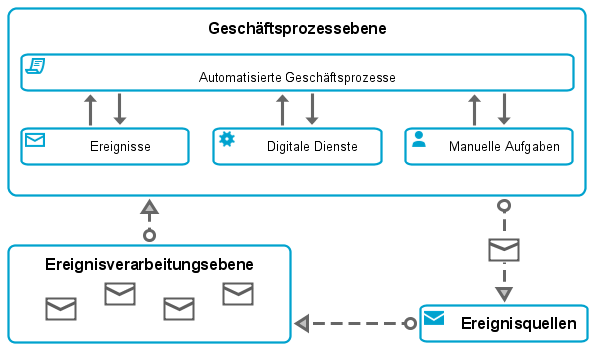
\includegraphics[width=\textwidth]{img/dynamicbp.png}	
    \caption[Ebenen dynamischer Geschäftsprozesse]
    {Ebenen dynamischer Geschäftsprozesse \protect\footnotemark}
    \label{fig:Ebenen dynamischer Geschäftsprozesse}
\end{figure}
\footnotetext{Eigene Darstellung, in Anlehnung an \citeauthor{Vidackovic.2014} \citeyear{Vidackovic.2014} \cite{Vidackovic.2014} }
\footnotetext{Die Abbildung dient lediglich der Visualisierung und ist nicht \ac{BPMN} 2.0 konform.}

Auf der Ereignisverarbeitungsebene werden eingehende Ereignisse aus diversen externen und internen Ereignisquellen kontinuierlich analysiert, wobei zudem Ereignisse generiert werden können, welche wiederum dieselbe Analyse durchlaufen. 
Da zwischen der Ereignisverarbeitungsebene und der Geschäftsprozessebene mit Ereignissen kommuniziert werden kann, können diese generierten Ereignisse als unmittelbare Reaktion eine dynamische Wirkung auf den Ablauf des laufenden Geschäftsprozess ausüben.
Der Geschäftsprozess fungiert demnach einerseits als eine der internen Ereignisquellen für die Ereignisverarbeitungsebene und andererseits als wesentlicher Ereigniskonsument der generierten Ereignisse zur Adaption des Prozessablaufs.
\cite{Benker.2016}

Auf der Geschäftsprozessebene erfolgt der operative und automatisierte Ablauf von Aktivitäten des Geschäftsprozesses, wobei Letztere in einer \ac{SOA} überwiegend auf elektronischen Diensten basieren, die als Webservices über standardisierte Schnittstellen aufgerufen werden und auch über Unternehmensgrenzen hinweg verteilt sein können.
\cite{Finger.2009}
Bei den Aktivitäten kann es sich darüber hinaus auch um manuelle Benutzeraufgaben handeln, die zwar von Menschen ausgeführt werden, aber dennoch mittels informationstechnischen Schnittstellen in einen automatisierten Prozessablauf integriert werden können.
\cite{Bruns.2010}


In ereignisorientierten im Gegensatz zu ablauforientierten Geschäftsprozessen üben Ereignisse zur Laufzeit einen signifikanten Einfluss auf den Prozessablauf aus, sodass die Geschäftsprozesse anhand geeigneter Ereignisverarbeitungsregeln mit dynamischen Eigenschaften ausgestattet werden können. 

\subsection{Gegenüberstellung vorhandener Forschungsansätze}
Die wesentlichen Aspekte der existierenden Forschungsansätze werden zunächst einzeln betrachtet und anschließend gegenübergestellt.

\paragraph{Entwicklung agiler Geschäftsprozesse mit Ereignisverarbeitung}
Dieser Forschungsansatz von \citeauthor{Alexopoulou.2008} aus dem Jahr \citeyear{Alexopoulou.2008} liefert eine Vorgehensweise zur Entwicklung dynamischer und ereignisgesteuerter Geschäftsprozesse, die nicht in Form eines abgeschlossenen Systems modelliert werden, sondern lediglich aus einzelnen Ereignis-Aktivität-Einheiten, sogenannten Dynamikeinheiten, bestehen. 
\cite{Alexopoulou.2008} 
Diese werden in Echtzeit auf der Ereignisverabreitungsebene ausgeführt und fügen den Geschäftsprozess dynamisch zusammen, wobei neue Ereignis-Aktivität-Einheiten bedarfsgerecht hinzugefügt werden können. 

Ein Defizit dieses Forschungsansatzes ist die fehlende Betrachtung des gesamten Ablaufs. Das Konzept dieser Dynamikeinheiten wird auch in dieser Bachelorarbeiten aufgegriffen, allerdings ausgehend von einem in seiner Gesamtheit modellierten Geschäftsprozess, der in diese Einheiten zerlegt wird.

\paragraph{RESTful SOA zur Automatisierung von Geschäftsprozessen}
Die Realisierung von \ac{SOA} in diesem Forschungsansatz von \citeauthor{Wolf.2016} ist in Übereinstimmung mit den Prinzipien von \ac{REST}. 
\footnote{
Da der technische Fokus in dieser Arbeit auf der Geschäftsprozessebene liegt, werden die einzelnen technischen Konzepte an dieser Stelle nicht weiter vertieft.
Für eine detaillierte Betrachtung der Prinzipien von \ac{REST} sei lediglich auf weiterführende Literatur verwiesen.
\cite{Wolf.2016}\cite{Masak.2007}\cite{Finger.2009}}
Die \ac{REST}ful \ac{SOA} entsteht durch den Entwurf serviceorientierter Architekturen gemäß den Bedingungen und Technologien von \ac{REST}. \ac{REST} ist ein Architekturstil für die Gestaltung verteilter Systeme, insbesondere bei der Umsetzung von Webservices. Durch dieses Vorgehen wird auf eine modellbasierte Spezifikation von \ac{REST}ful \ac{SOA} für die Automatisierung von Geschäftsprozessen abgezielt. \cite{Wolf.2016}

Insbesondere die Überwindung der semantischen Lücke zwischen Geschäftsprozessmodell und Anwendungssystem durch ein systematisches Vorgehen wird in diesem Forschungsansatz behandelt. Die identifizierten Probleme werden durch einen Ansatz zur Konzeption eines Anwendungssystems auf Basis von auf fachlicher Ebene modellierten Geschäftsprozessen angegangen.  
Es fehlen allerdings Möglichkeiten zur Modellierung wesentlicher Konzepte der Echtzeitverarbeitung von Ereignissen.
Da der Forschungsansatz wohl aber auf die automatisierte Ausführung von Geschäftsprozessen mithilfe von digitalen Diensten ausgerichtet ist, bleibt der Ansatz für die softwaretechnische Implementierung in Kapitel von Relevanz. 

\paragraph{Methodology for Business Dynamics\textsuperscript{dbpm}}
Der Forschungsansatz von \citeauthor{Vidackovic.2014} stellt die  Methode [moby]\textsuperscript{dbpm} zur Entwicklung dynamischer Geschäftsprozesse mit Ereignisverarbeitung dar. Der Name [moby]\textsuperscript{dbpm} steht dabei für Methodology for Business Dynamics und dbpm für Dynamic Business Process Management. Der Ansatz bietet einen geeigneten Lösungsansatz für die Problemstellung dynamischer Geschäftsprozesse mit Ereignisverabeitung an und stellt das dafür benötigte, webbasierte Modellierungswerkzeug zur Verfügung. 
\cite{Vidackovic.2014}

Die Modellierung wird in einer von \citeauthor{Vidackovic.2014} erweiterten Form von \ac{BPMN} 2.0 vorgenommen. Des Weiteren folgt der Ansatz den Konzepten der modellbasierten Softwarentwicklung. Die Geschäftsprozessmodelle können in Kombination mit dem Produkt \textit{Esper} mit Code angereichert und anschließend automatisch ausgeführt werden ohne eine weitere Implementierung in ein Anwendungssystem. Der Ansatz einer modellbasierten Softwarentwicklung wird im Rahmen dieser Bachelorarbeit, aufgrund mangelnder Integrationsmöglichkeiten mit SAP S/4HANA Cloud, nicht weiter verfolgt. Die Ergebnisse des Forschungsansatzes von \citeauthor{Vidackovic.2014} werden jedoch als wertvoller Beitrag in diesem Fachbereich angesehen.  

\paragraph{SOEDA-Methode}
SOEDA beschreibt ein Verfahren zur Entwicklung von Anwendungssystemen durch die Zusammenführung von serviceorientierten (SOA) und ereignisgesteuerten Architekturen (EDA). Geschäftsprozesse werden hier mit \ac{EPK}s modelliert. 
\cite{MatthiasWieland.2009} 
Mit Hilfe von grafischen Modellierungswerkzeugen werden die zugrunde liegenden Aktivitäten modularisiert und mit entsprechenden Ereignissen gekoppelt, so dass ein Entwickler die Regeln der Ereignisverarbeitung anschließend in einer spezifischen Programmiersprache implementieren kann. 
\cite{Bruns.2010}

Schwächen der SOEDA-Methode sind die unzureichende Modellierung von Ereignisverarbeitungsregeln durch die Verwendung von \ac{EPK}s. 
\cite{RobraBissantz.2009}
Auch mangelt es an der Abbildung von Ereignissen im Geschäftsprozess, da Ereignisse nur als Teil des normalen Geschäftsprozessablaufs betrachtet werden. Mit der Version 2.0 verfügt die \ac{BPMN}, wie in Abschnitt \ref{sec:Automatisierung} erwähnt, nun nicht nur über eine grafische Notation, sondern auch über die Semantik der technischen Ausführung. Auf \ac{EPK}s kann demzufolge im Rahmen der Bachelorarbeit verzichtet werden, zumal eine Konsistenz des Geschäftsprozessmodells auf betriebswirtschaftlicher und technischer Ebene wünschenswert ist.

\paragraph{Gegenüberstellung der Ansätze}
Auf Basis der Darstellung der existierenden Forschungsansätze wird ersichtlich, dass die bestehenden Forschungsansätze für die Anreicherung von Geschäftsprozessmodellen mit Konzepten der Ereignisverarbeitung jeweils einen bestimmten Fokus besitzen, dessen Herausforderungen im Einzelfall ausreichend erfüllt werden. 
Eine Kopplung von Ereignissen und Aktivitäten mithilfe des Ansatzes von \citeauthor{Alexopoulou.2008}, fachliche Aspekte wie die der SOEDA-Methode, die technischen Möglichkeiten der \enquote{RESTful SOA} oder eine automatisierte Ausführung der [moby]\textsuperscript{dbpm} finden beispielsweise keine Betrachtung. 

Folglich lässt sich sagen, dass bisher noch kein Lösungsansatz mit einer ganzheitlichen und durchgängigen Vorgehensweise existiert, die eine vollständige, formale sowie fachlich orientierte Modellierung von Geschäftsprozessen mit dynamischen Eigenschaften auf Basis von Ereignisverarbeitung ermöglicht.

